% !TeX root = ../thesis.tex
\section{Areas of Use}

%TODO: Performance
\begin{figure} 
	\centering
	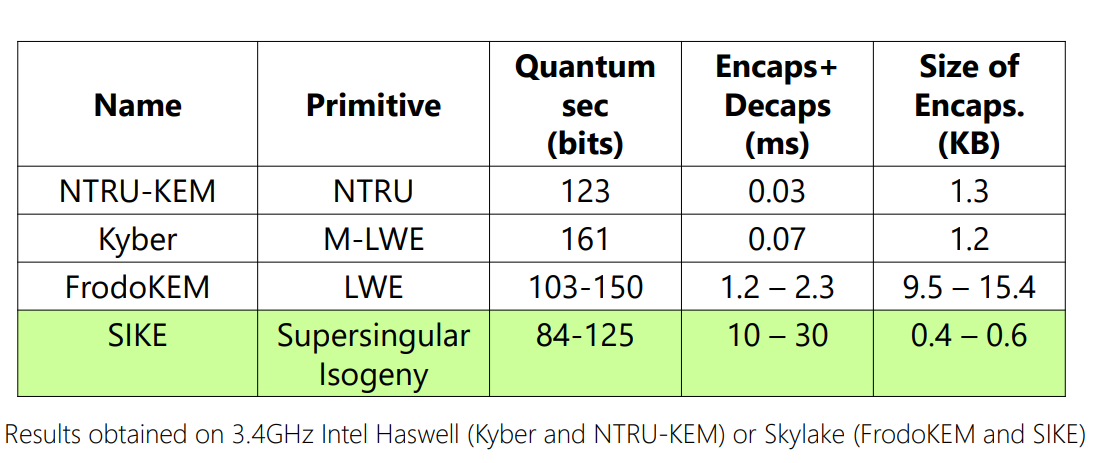
\includegraphics[width=1\linewidth]{../img/performance}
	\caption{SIKE performance in comparison}
	\label{fig:performance}
\end{figure}

SIDH features some of the lowest key sizes among all NIST PQC competition candidates. Unfortunately, it's performance is also up to a factor of 100 worse than the best alternative, as shown in figure \ref{fig:performance}.


Due to the low key sizes SIDH is perfectly suited for deployment in applications where space is limited, e.g. in protocols such as Bitcoin or Tor, where the maximum data cell size is 517 bytes, which fits a SIDH key, but would be too big for NTRUEncrypt, as an example. On the other hand, due to the high computational complexity of computing keys, SIDH has some disadvantages in comparison to other post-quantum protocols if used in embedded devices.